\section{Implementation and Performance Assessment}


CCVPN is implemented as a network layer service running on the gateways of private networks that compose the VPN (see Fig.\ref{fig:ccvpn}).
Our implementation uses the CCNx software stack~\cite{CCNxGithub} and the cryptographic library Sodium~\cite{sodiumGithub}. These are both publicly available and written in C.
For the PKE version of CCVPN, interest encapsulation and decapsulation routines (Alg.~\ref{alg:interestEncap}, and . Alg.~\ref{alg:interestDecap}) are implemented using \todo{check alg} as public key
encryption (and decryption) algorithm. \todo{check alg} is used to encrypt-then-MAC the content reponses (Alg.~\ref{alg:contentEnc}, and Alg.~\ref{alg:contentDec}). Recall that the symmetric keys used by
\todo{check alg} are generated and sent together with the encapsulated interest in Alg.~\ref{alg:interestEncap}.
In the symmetric key version of the design, \todo{check alg} was used to encrypt-then-MAC both, interests and contents.



In this section we empirically evaluate the CCVPN design paying special attention to the metrics that were earlier discussed in Sec.~\ref{sec:analysis}, i.e., processing overhead, network throughput, and state consumption. In our evaluation we consider the two versions of CCVPN: public key version, and symmetric key version. We here recall that the symmetric key version relies on the assumption that a secure key agreement protocol is performed between the domain's gateways prior to the CCVPN protocol execution.

Our testbed network consists of a butterfly topology, in which the consumers' side and the producers' side gateways are directly interconnected. $N$ producers are connected to the producers' domain gateway and $M$ consumers are connected to the consumers' domain gateway (see Fig.~\ref{create_figure}).

To investigate the processing overhead we measure the average time demand for computing the interests' encapsulation (in public and symmetric key versions), interest decapsulation, content encryption, and content decryption for different content packet sizes (1024, 4096, 16384, and 65536 bytes). We also measure the state consumption for these same four functions.

To compute the overall network throughput we measure the average data-rate for transmissions of 1 to 1,000,000 different interests issues per consumer. We also vary the number of consumers and producers from 1 to 10 of each. Finally, in addition to the network throughput, we also exhibit the total transmission delay for each of the experiments.

\todo{TODO: Add results discussion}

\begin{table}[!h]
\centering
\caption{Interest encapsulation processing times}
\label{my-label}
\begin{tabular}{|l|l|l|l|l|}
\hline
Encapsulation mode   & Encapsulation & Decapsulation \\ \hline
Public Key  & 444$\mu s$           & 449$\mu s$           \\ \hline \cline{4-5} 
Symmetric Key & TODO          & TODO          \\ \hline
\end{tabular}
\end{table}



\begin{table}[!h]
\centering
\caption{Content encryption and decryption times for different payload sizes}
\label{my-label}
\begin{tabular}{|l|l|l|}
\hline
Packet size        & Encryption & Decryption \\ \hline
$1024$B & 125$\mu s$        & 193$\mu s$        \\ \hline
$4096$B & 141$\mu s$        & 220$\mu s$        \\ \hline
$16384$B & 220$\mu s$        & 367$\mu s$        \\ \hline
$65536$B & 519$\mu s$        & 702$\mu s$        \\ \hline
\end{tabular}
\end{table}

\begin{figure}[]
\centering
  \subfigure[Throughput]{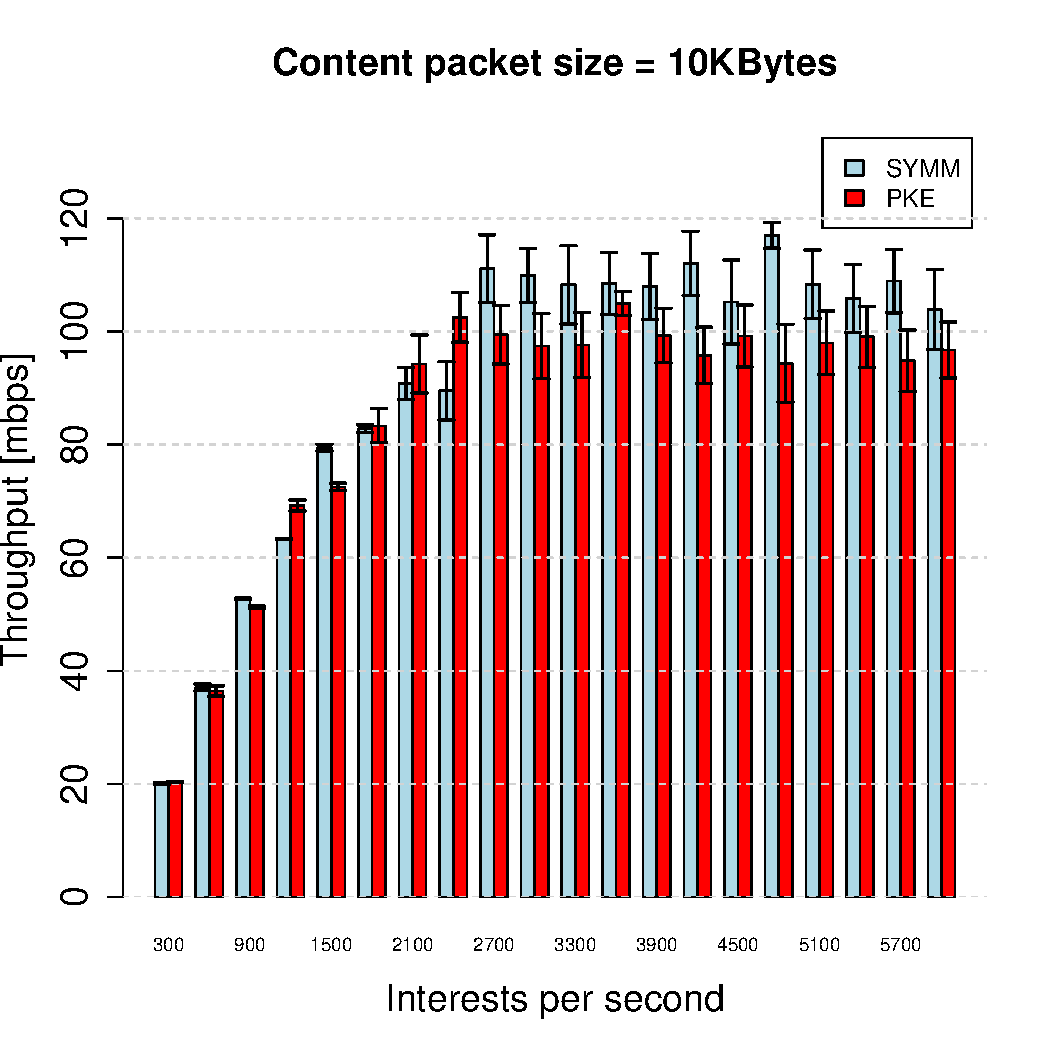
\includegraphics[width=0.49\columnwidth]{images/1_1_thput.pdf}\label{1a}}
  \hfil
  \subfigure[Avg. RTT]{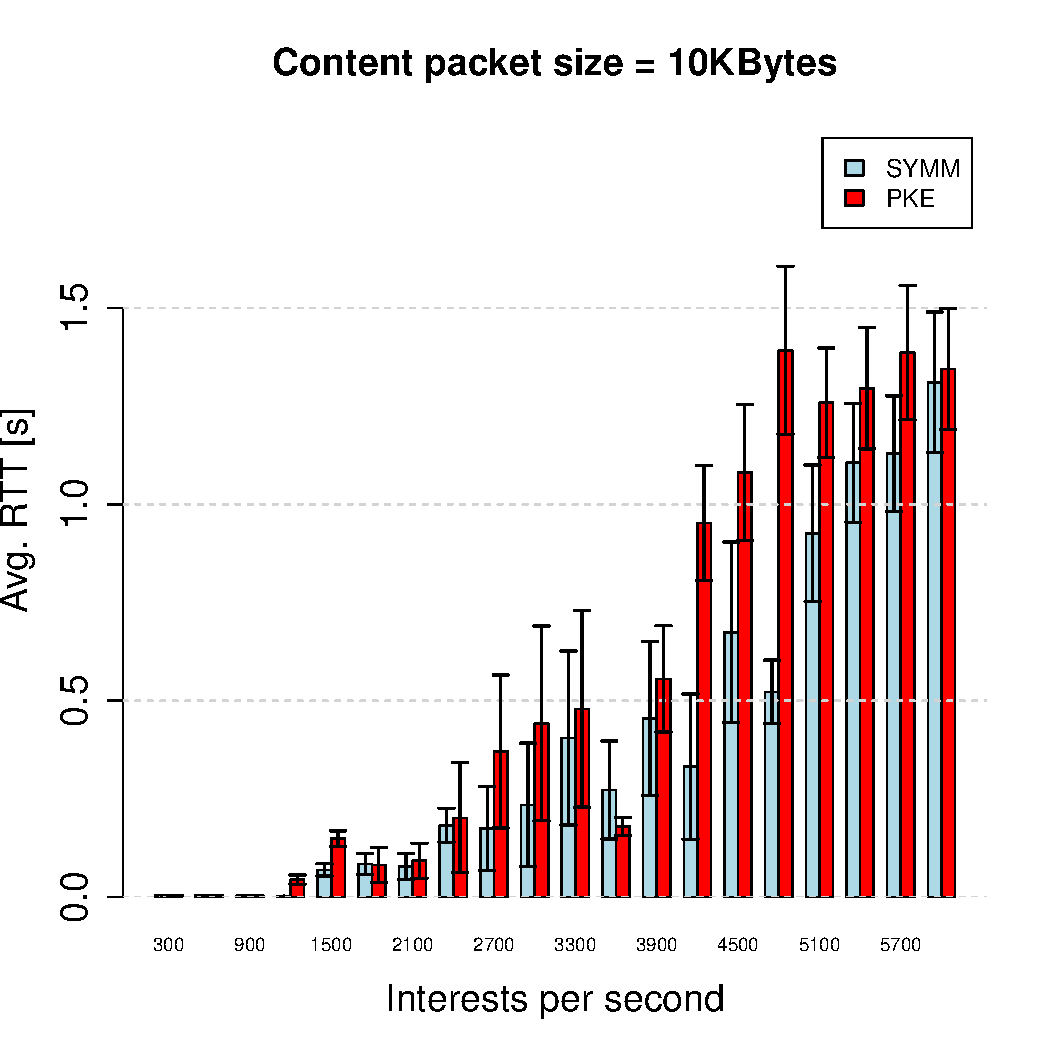
\includegraphics[width=0.49\columnwidth]{images/1_1_rtt.pdf}\label{1b}}
\caption{CCVPN performance with one consumer and one producer for increasing interest issuance rates.}\label{exp1}
\end{figure}

\begin{figure}[]
\centering
  \subfigure[Throughput]{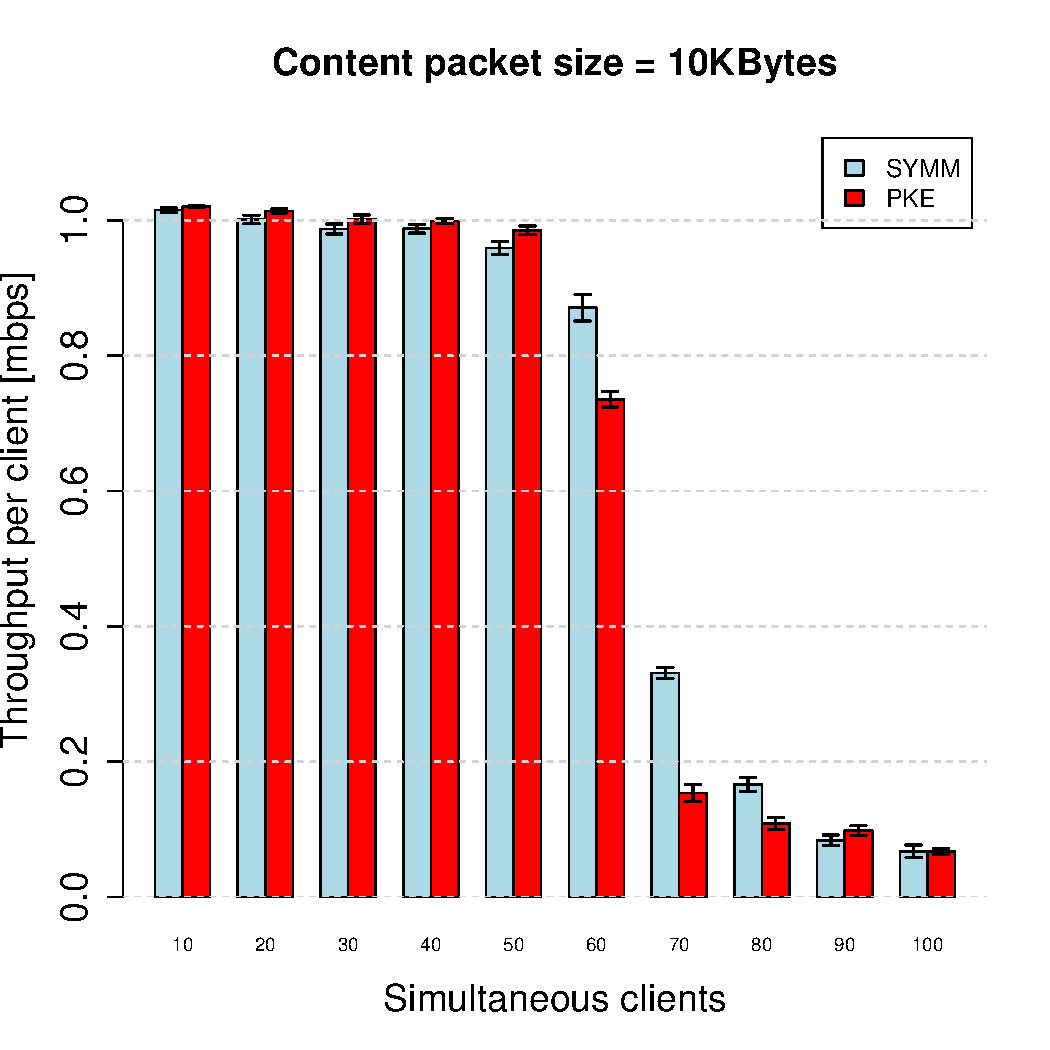
\includegraphics[width=0.49\columnwidth]{images/n_1_thput.pdf}\label{1a}}
  \hfil
  \subfigure[Avg. RTT]{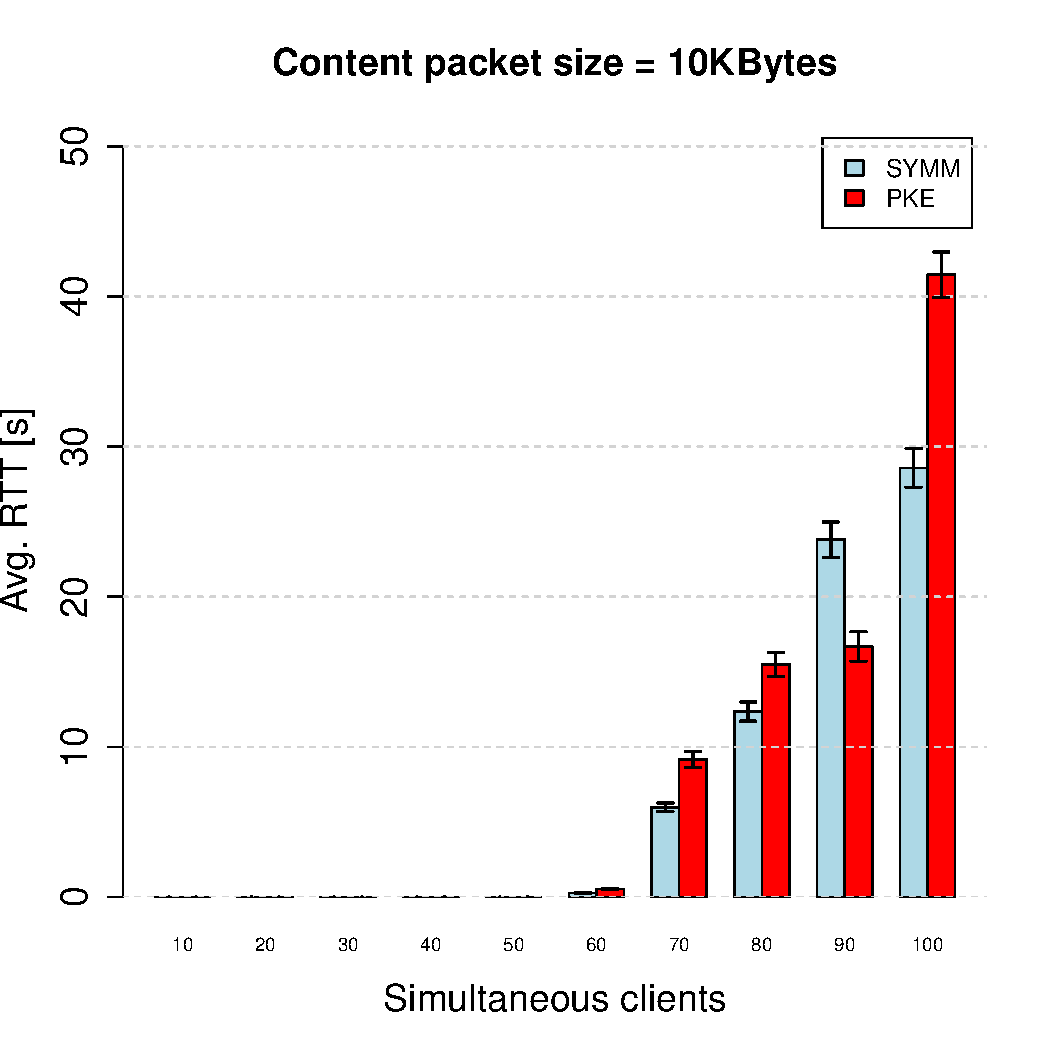
\includegraphics[width=0.49\columnwidth]{images/n_1_rtt.pdf}\label{1b}}
\caption{CCVPN performance with multiple consumers and one producer. Each consumer requests with 1 mbps rate.}\label{exp1}
\end{figure}

\begin{figure}[]
\centering
  \subfigure[Throughput]{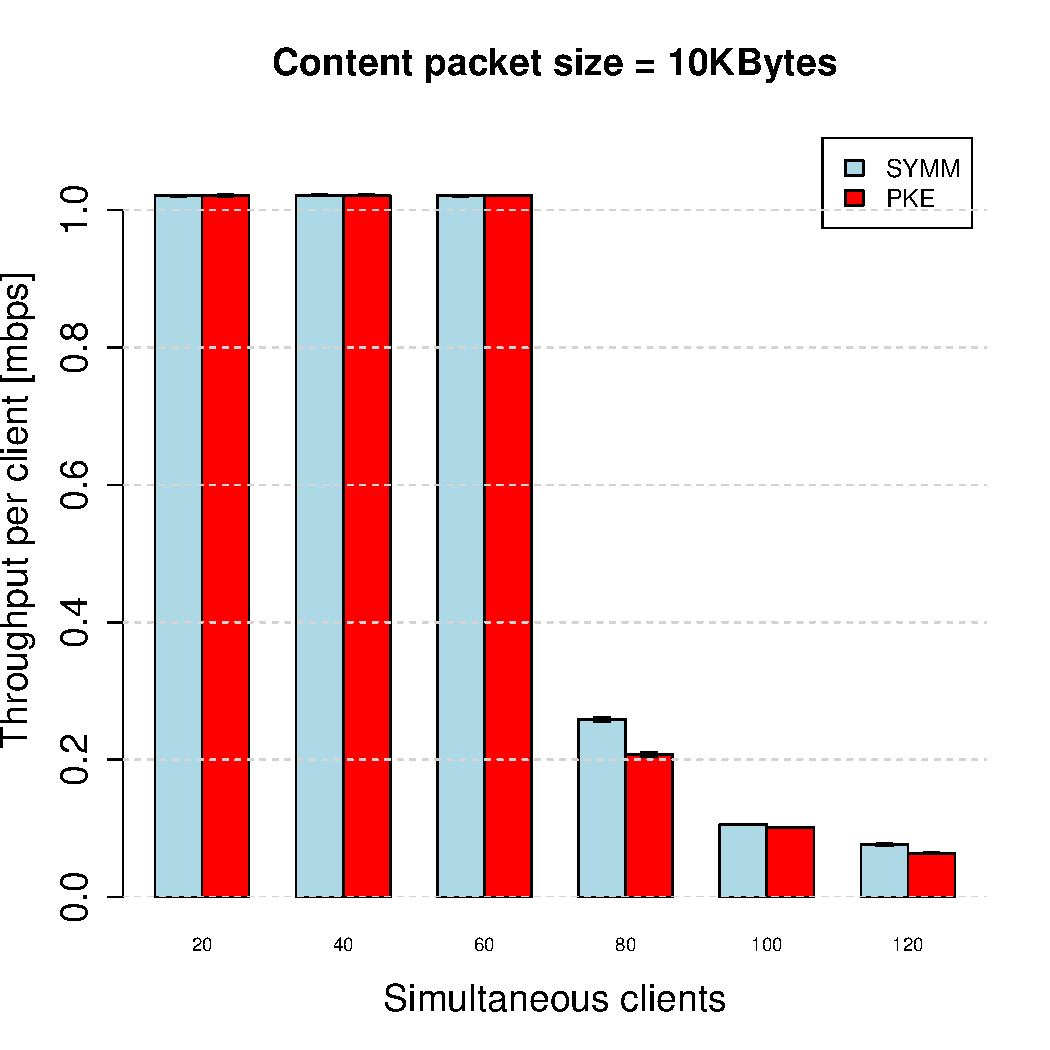
\includegraphics[width=0.49\columnwidth]{images/n_n_thput.pdf}\label{1a}}
  \hfil
  \subfigure[Avg. RTT]{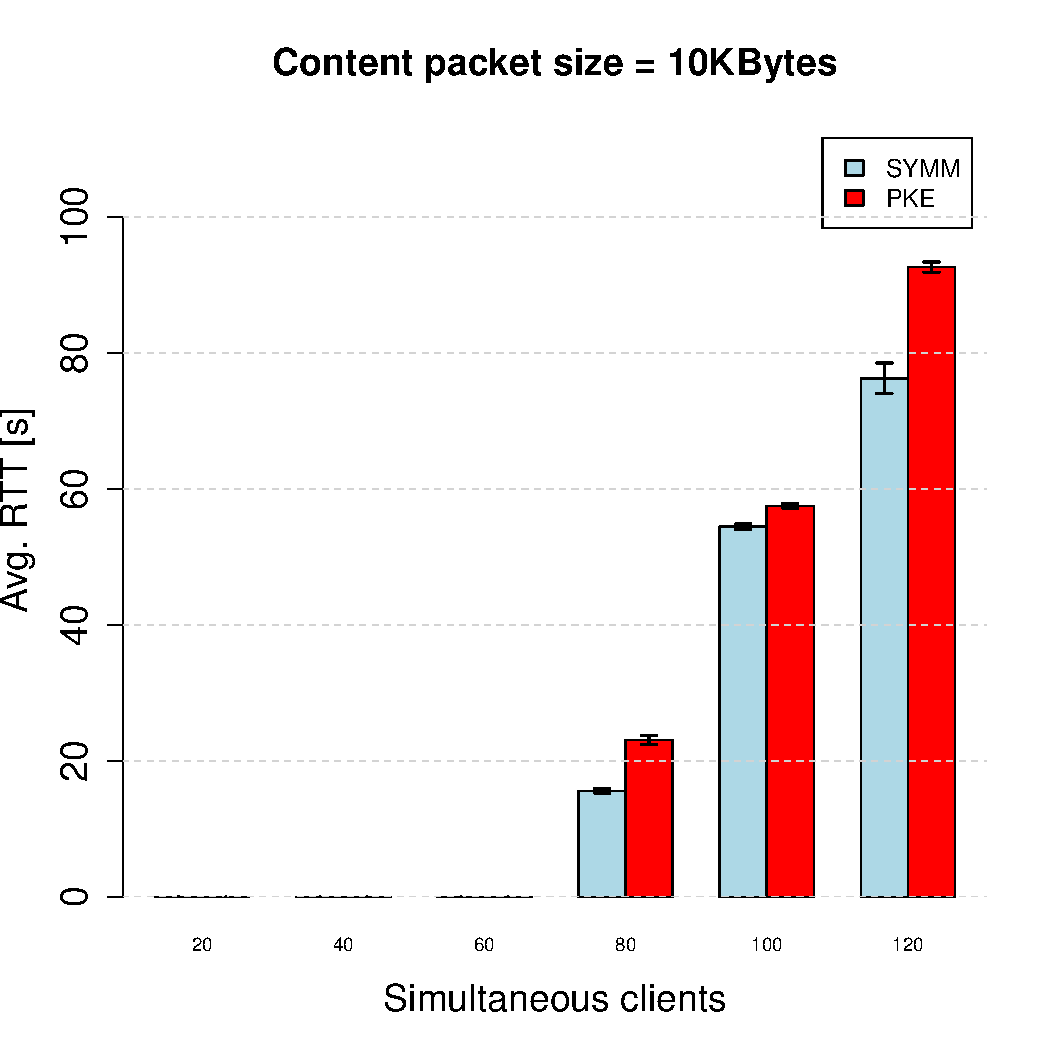
\includegraphics[width=0.49\columnwidth]{images/n_n_rtt.pdf}\label{1b}}
\caption{CCVPN performance with multiple consumers and multiple producers. Each consumer requests with 1 mbps rate.}\label{exp1}
\end{figure}



